\subsection{Missclassifications}
\label{sec:predictions-misclassifications}
%0-4
%bathtub_0117_2_006.png as 0 small feature
%bathtub_0125_3_004.png as 1 red only small, never complete, if triangle then truncated and small
%bathtub_0127_1_007.png as 3 in red as 0, small feature, prefers green
%in general small but long features are misclassified
%
%0-5
%0117_2 as 0 again
%mostly 1 as 4 predicted
%
%0-6
%0117_5 as 2 small feture
%
%4-0
%bathtub_0111_0_011.png as sofa no sharp shadow could look like a sofa // in every 4-* network but other material
%
%4-*
%similar multi-views in all in particular bathtub->sofa
%dresser_0215_2_010.png as dresser_0 very small feature
%sofa_0685_1_011.png as sofa_0 very small feature
%4-5
%sofa_0681_1_010.png as dresser 4
By comparing all misclassifications of all networks several similarities are found.
It is noticed that an object with a wrong prediction is likely to reappear across different networks.
Not always with the exact same material, though, but this could be due to different weight initializations.
The most common reason for predicting a wrong class within the same object category are small features.
Some examples are shown in \figref{fig:small-features}.
\begin{figure}
	\centering
	\begin{subfigure}{.3\textwidth}
		\centering
		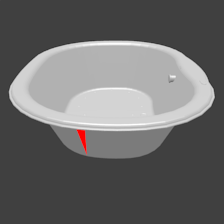
\includegraphics[width=.8\textwidth]{images/bathtub_0117_2_006.png}
		\caption{Predicted as Blank}
		\label{fig:small-features-a}
	\end{subfigure}
	%
	\begin{subfigure}{.3\textwidth}
		\centering
		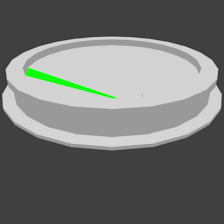
\includegraphics[width=.8\textwidth]{images/bathtub_0127_1_007.png}
		\caption{Predicted as Green-Red}
		\label{fig:small-features-b}
	\end{subfigure}
	%
	\begin{subfigure}{.3\textwidth}
		\centering
		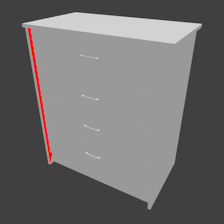
\includegraphics[width=.8\textwidth]{images/dresser_0215_2_010.png}
		\caption{Predicted as Blank}
		\label{fig:small-features-c}
	\end{subfigure}
	
	\begin{subfigure}{.3\textwidth}
		\centering
		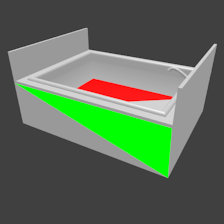
\includegraphics[width=.8\textwidth]{images/bathtub_0125_3_004.png}
		\caption{Predicted as Green}
		\label{fig:small-features-d}
	\end{subfigure}
	%
	\begin{subfigure}{.3\textwidth}
		\centering
		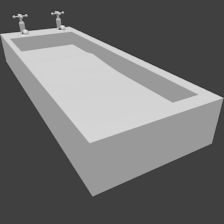
\includegraphics[width=.8\textwidth]{images/bathtub_0111_0_011.png}
		\caption{Predicted as Blank Sofa}
		\label{fig:small-features-e}
	\end{subfigure}
	%
	\begin{subfigure}{.3\textwidth}
		\centering
		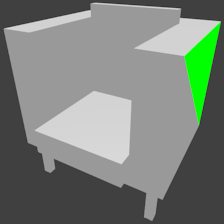
\includegraphics[width=.8\textwidth]{images/sofa_0681_1_010.png}
		\caption{Predicted as Green-Green Dresser}
		\label{fig:small-features-f}
	\end{subfigure}
	\caption[Reasons for Incorrect Predictions]{Reasons for incorrect predictions are small features, hidden features and missing shadows.}
	\label{fig:small-features}
\end{figure}
The first multi-view is often predicted as blank and the second one as green-red.
Why the material color is predicted wrong, however, remains unknown.
Similar object are found in the dataset which are predicted wrong that have features of a similar size like \figref{fig:small-features-c}.
For the fourth one the red face is never seen completely, hence, it is never seen in a triangular shape like usual material faces except for one view.
There it is truncated to a small triangular, though, and experiences the same problems as the other two multi-views presumably.
Two optimal faces next to each other forming a rectangle result in a correct classification in general, however.
The case of two faces building a larger triangle is not present in the dataset.
Although it is assumed that such a multi-view would be predicted wrong.
The reason for predicting bathtubs incorrectly as sofas are mostly missing shadows like in \figref{fig:small-features-e}.
Because mainly the long left side transitions into the plane due to a missing sharp shadow at the edge the actual bathtub is more likely to be predicted as a sofa.
This object is indeed likely to reappear in different networks as a wrong prediction.
However, the actual and predicted material differs.
\figref{fig:small-features-f} is classified as a dresser with a green-green material feature.
Though, it is a sofa and has only one green material feature.
This shows that many multi-views are just predicted wrong without an interpretable or obvious cause.